% !TeX program = xelatex
\documentclass[12pt,a4paper]{exam-zh}

\usepackage{amsmath,array,graphicx,booktabs,multirow}
\usepackage{enumitem}
\usepackage{fancyhdr}
\usepackage{tikz}
\usepackage{tabularx}
\usepackage{setspace}
\setCJKmainfont{Noto Serif CJK SC}
\geometry{margin=2.2cm,top=2.0cm,bottom=2.2cm}
\pagestyle{fancy}
\fancyhf{}
\cfoot{-\thepage{}-}
\renewcommand{\headrulewidth}{0pt}
\renewcommand{\footrulewidth}{0pt}
\setlength{\parindent}{0pt}
\setlength{\parskip}{0.2em}
\setlength{\headheight}{14pt}
\linespread{1.12}
\usepackage{setspace}
\usepackage{eso-pic}
\usetikzlibrary{calc,arrows.meta}

%region exam setup

\examsetup{
    page = {
    size = a4paper,           % 设定纸张大小 [4]
    foot-content = { - ; - }  % 页脚显示为 -1-, -2- 格式 [3]
  },
    choices = {
    label-pos = top-left,
    column-sep = 1em,
    label-pos = auto,
    label-sep = 0.5em,
    max-columns = 4
    },
  question = {
    top-sep    = 1em, % 调整题目上方的垂直距离（默认值为 .5em plus .5em minus .2em）
    bottom-sep = 1em  % 调整题目下方的垂直距离（默认值为 .5em plus .5em minus .2em）
  },
    paren = {
    show-paren = false  % 设置为 false 则不显示括号 [3, 4]
  },
    choices = {
    label = \textbf{\Alph*}
  }, 
    solution = {
    show-solution = show-move, % 答案自动移动到卷末
    label-content = {参考答案},  % 答案区的标题文字
    show-qed = true            % 在解答末尾显示结束符号 ◻ 
  }
}

%endregion


%region 卷面变量设置
    % ==========================
    % 兼容从当前文件夹或工作区根目录进行编译
    % ==========================
% 卷面变量设置（只需改这里）
% ==========================
\newcommand{\papercode}{SC 07}
\newcommand{\examtitle}{2026年金宝培元独立中学毕业考}
\newcommand{\examlevel}{高中组}
\newcommand{\examsubject}{高级数学(I)}
\newcommand{\sidebartext}{高级数学(I)/一}
\newcommand{\papername}{试卷一}
\newcommand{\papertype}{选择题}
\newcommand{\examdate}{2026年9月24日}
\newcommand{\examtime}{8.00 a.m.－9.00 a.m.}
\newcommand{\examduration}{60分钟}
\newcommand{\questionpages}{4面}
\newcommand{\paperonepercentage}{30\%}
\newcommand{\papertwopercentage}{70\%}
\newcommand{\setterteacher}{蔡杰庆师}
\newcommand{\reviewteacher}{杨丽芳师}
\newcommand{\auditteacher}{雷泳健师}


    \newcommand{\optrow}[4]{%
    \begin{tabular*}{\linewidth}{@{\extracolsep{\fill}}llll}
    A~#1 & B~#2 & C~#3 & D~#4
    \end{tabular*}%
    }
    \newcommand{\qitem}[5]{\item #1\par\optrow{#2}{#3}{#4}{#5}}
%endregion
    \begin{document}


%region 封面
    \AddToShipoutPictureFG*{%
    \begin{tikzpicture}[remember picture,overlay]
        \node[
            anchor=north west,
            fill=black,
            minimum width=22pt,
            minimum height=90pt,
            inner sep=0pt
        ] (sidebar) at ([xshift=3em,yshift=-3em]current page.north west) {};
        \node[
            rotate=270,
            text=white,
            font=\bfseries\footnotesize
        ] at (sidebar.center) {\sidebartext};
    \end{tikzpicture}%
    \put(24,18){\makebox(0,0)[lb]{\small 版权所有}}%
    \put(520,18){\makebox(0,0)[lb]{\bfseries\small 【机密】}}%
    }

    \thispagestyle{fancy}

    \begin{minipage}[t]{0.22\linewidth}
    \vspace{0pt}
    \end{minipage}
    \hfill
    \begin{minipage}[t]{0.8\linewidth}
        \centering
        {\zihao{2}\bfseries \examtitle\par}
        \vspace{1.3em}
        {\zihao{3}\bfseries \examlevel\par}
        \vspace{1.3em}
        {\zihao{2}\bfseries \examsubject\par}
        \vspace{0.2em}
        {\large (\papercode)\par}
    \end{minipage}
    \hfill
    \begin{minipage}[t]{0.18\linewidth}
    \vspace{0pt}
    \end{minipage}

    \vspace{3.0em}

    \begin{center}
    \begin{tabular}{l}
        \multicolumn{1}{c}{\papername\hspace{2em}\papertype}\\[-0.1em]
        \midrule
        日期：\examdate\\[-0.1em]
        时间：\examtime\\[-0.1em]
        \multicolumn{1}{c}{(\examduration)}\\
        \midrule
    \end{tabular}
    \end{center}

    \vspace{2.0em}

    {\zihao{4}\bfseries \underline{考生须知}\par}
    \vspace{0.8em}

    \begin{enumerate}[label=（\chinese*）,leftmargin=3em,itemsep=0.65em]
    \item 本科试卷共分两份：\\
    \hspace*{2em}试卷一：选择题（\paperonepercentage）；\\
    \hspace*{2em}试卷二：作答题（\papertwopercentage）。

    \item 考生须于第一阶段规定的60分钟内完成试卷一。第二阶段规定的2小时内作答试卷二。

    \item 试卷一选择题20题全答。选出正确的答案，然后用\textbf{5B铅笔将“O”答案纸}（电脑卡）上相应的字母所在的小方格涂黑。

    \item 可使用电子计算机进行演算。

    \item 试卷一选择题共印\questionpages。
    \end{enumerate}

    \vspace{2.0em}

    \begin{center}
    {% 外框粗细及外、内框之间的距离
    \setlength{\fboxrule}{3pt}%
    \setlength{\fboxsep}{1.5pt}%
    \fbox{%
        {% 内框粗细及文字与内框之间的距离
        \setlength{\fboxrule}{0.5pt}%
        \setlength{\fboxsep}{6pt}%
        \fbox{\rule{0pt}{1.1em}\hspace{1.2em}{\zihao{4}\bfseries 未经正式宣布\quad 不得翻看内页}\hspace{1.2em}}%
        }%
    }%
    }
    \end{center}

    \vfill

    \begin{tabular*}{\linewidth}{@{\extracolsep{\fill}}ll}
    考生姓名：\underline{\hspace{4.2cm}} & 考生编号：\underline{\hspace{4.0cm}}
    \end{tabular*}

%endregion

\newpage
%region 范围：三角函数与直线方程的综合应用 | 考点：三角函数符号判断、直线斜截式与象限分布 | 难度：中等
\begin{question}
    已知 $\theta$ 为第三象限角，则直线 $x\sin\theta + y\cos\theta = \tan\theta$ 一定不经过哪个象限？ \paren[A]
    \begin{choices}
        \item 第一象限
        \item 第二象限
        \item 第三象限
        \item 第四象限
    \end{choices}
\end{question}

\begin{solution}
    判断直线 $x\sin\theta+y\cos\theta=\tan\theta$（$\theta$ 为第三象限角）不经过哪个象限。\\
    由第三象限角性质得 $\sin\theta<0,\ \cos\theta<0,\ \tan\theta>0$，将直线化为斜截式后分析斜率与截距的正负。\\
    \begin{align*}
        y &= \dfrac{\tan\theta-x\sin\theta}{\cos\theta} \\
        &= -\dfrac{\sin\theta}{\cos\theta}x+\dfrac{\sin\theta}{\cos^2\theta}
    \end{align*}
    斜率 $k=-\tan\theta<0$，截距 $b=\dfrac{\sin\theta}{\cos^2\theta}<0$（因 $\sin\theta<0,\ \cos^2\theta>0$）。
    \[
        k<0,\ b<0 \implies \text{直线经过第二、三、四象限，不经过第一象限}
    \]
    故选 A。
\end{solution}
%endregion
%region 范围：高中代数——多项式因式的代入验根判断 | 考点：利用 $x^k=-1$ 代入验证多项式因式 | 难度：困难
\begin{question}
    下列何者不是 $x^{48}-4x^{12}+3$ 的因式？ \paren[D]
    \begin{choices}
        \item $x+1$
        \item $x^{2}+1$
        \item $x^{3}+1$
        \item $x^{4}+1$
    \end{choices}
\end{question}

\begin{solution}
    判断 $x+1,\ x^2+1,\ x^3+1,\ x^4+1$ 中何者不是 $x^{48}-4x^{12}+3$ 的因式。\\
    形如 $x^k+1$ 的因式其根满足 $x^k=-1$，代入原式判断结果是否为零即可，无需展开因式分解。\\
    设各选项对应的根满足 $x^k=-1$（$k=1,2,3,4$），则 $x^{12}=(x^k)^{\frac{12}{k}}=(-1)^{\frac{12}{k}}$。
    \begin{align*}
        k=1:\ x^{12}&=(-1)^{12}=1, &x^{48}-4x^{12}+3 &= 1-4+3=0 \\
        k=2:\ x^{12}&=(-1)^{6}=1, &x^{48}-4x^{12}+3 &= 1-4+3=0 \\
        k=3:\ x^{12}&=(-1)^{4}=1, &x^{48}-4x^{12}+3 &= 1-4+3=0 \\
        k=4:\ x^{12}&=(-1)^{3}=-1, &x^{48}-4x^{12}+3 &= 1+4+3=8
    \end{align*}
    唯有 $k=4$ 时代入结果不为零，即 $x^4+1$ 不能整除 $x^{48}-4x^{12}+3$。
    故选 D。
\end{solution}
%endregion

%region 范围：高中函数——复合函数化简与反函数求值 | 考点：由复合函数表达式还原原函数、反函数定义式的求解与代入计算 | 难度：基础
\begin{question}
    已知函数 $f(3x+2)=6x+1$，求 $f^{-1}(-7)$ 的值。 \paren[A]
    \begin{choices}
        \item $-2$
        \item $2$
        \item $-5$
        \item $5$
    \end{choices}
\end{question}

\begin{solution}
    已知 $f(3x+2)=6x+1$，求 $f^{-1}(-7)$ 的值。\\
    先设 $u=3x+2$ 还原出 $f(x)$ 的表达式，再由 $y=f(x)$ 反解出 $x$ 得到反函数，最后代入 $y=-7$ 求值。\\
    设 $u=3x+2$，则 $x=\dfrac{u-2}{3}$。
    \begin{align*}
        f(u) &= 6\cdot\dfrac{u-2}{3}+1 \\
        &= 2(u-2)+1 \\
        &= 2u-3
    \end{align*}
    即 $f(x)=2x-3$。设 $y=2x-3$，反解 $x$：
    \begin{align*}
        y &= 2x-3 \\
        x &= \dfrac{y+3}{2}
    \end{align*}
    即 $f^{-1}(y)=\dfrac{y+3}{2}$，代入 $y=-7$：
    \[
        f^{-1}(-7) = \dfrac{-7+3}{2} = -2
    \]
    故选 A。
\end{solution}
%endregion

%region 范围：高中代数——不等式（分式不等式） | 考点：分式不等式转化为整式不等式后的符号法则与临界点取舍（含等号临界点与定义域排除点的区分） | 难度：中等偏难
\begin{question}
    求不等式 $\dfrac{2x-1}{x-3}\geq1$ 的解集。 \paren[A]
    \begin{choices}[columns=2,linesep=0pt]
        \item $(-\infty,-2]\cup(3,+\infty)$
        \item $[-2,3)$
        \item $(-\infty,-2)\cup(3,+\infty)$
        \item $(-\infty,-2]\cup[3,+\infty)$
    \end{choices}
\end{question}

\begin{solution}
    求不等式 $\dfrac{2x-1}{x-3}\geq1$ 的解集。\\
    移项通分转化为同一分式与 $0$ 比较，再对分子分母乘积作符号分析（不可直接两边乘 $x-3$）。
    \begin{align*}
        \dfrac{2x-1}{x-3}-1 &\geq0 \\
        \dfrac{2x-1-(x-3)}{x-3} &\geq0 \\
        \dfrac{x+2}{x-3} &\geq0
    \end{align*}
    由符号法则，$x+2$ 与 $x-3$ 同号或 $x+2=0$（须 $x-3\neq0$），临界点为 $x=-2,\ x=3$：
    \[
        x\leq-2 \ \text{或} \ x>3
    \]
    故选 A。
\end{solution}
%endregion

%region 范围：高中三角函数——半角公式与二倍角关系的综合运算 | 考点：半角公式 $\sin^2\frac{\theta}{2}=\frac{1-\cos\theta}{2}$、二倍角展开 $(\cos\frac{\theta}{2}-\sin\frac{\theta}{2})^2$ 及由和求积的对称式化简 | 难度：中等
\begin{question}
    已知 $\sin\theta+\cos\theta=\dfrac{1}{2}$，则 $\sin^{2}\dfrac{\theta}{2}\left(\cos\dfrac{\theta}{2}-\sin\dfrac{\theta}{2}\right)^{2}$ 的值为 \paren[A]
    \begin{choices}
        \item $\dfrac{1}{16}$
        \item $\dfrac{1}{8}$
        \item $\dfrac{7}{16}$
        \item $-\dfrac{1}{16}$
    \end{choices}
\end{question}

\begin{solution}
    已知 $\sin\theta+\cos\theta=\dfrac{1}{2}$，求 $\sin^{2}\dfrac{\theta}{2}\left(\cos\dfrac{\theta}{2}-\sin\dfrac{\theta}{2}\right)^{2}$ 的值。\\
    先将 $\left(\cos\frac{\theta}{2}-\sin\frac{\theta}{2}\right)^2$ 用二倍角公式化为 $1-\sin\theta$，再结合半角公式 $\sin^2\frac{\theta}{2}=\frac{1-\cos\theta}{2}$ 化为关于 $\sin\theta,\cos\theta$ 的对称式代入求值。
    \begin{align*}
        \left(\cos\dfrac{\theta}{2}-\sin\dfrac{\theta}{2}\right)^{2} &= \cos^2\dfrac{\theta}{2}-2\sin\dfrac{\theta}{2}\cos\dfrac{\theta}{2}+\sin^2\dfrac{\theta}{2} \\
        &= 1-\sin\theta
    \end{align*}
    \begin{align*}
        \sin^{2}\dfrac{\theta}{2}\left(\cos\dfrac{\theta}{2}-\sin\dfrac{\theta}{2}\right)^{2} &= \dfrac{1-\cos\theta}{2}\cdot(1-\sin\theta) \\
        &= \dfrac{1-\sin\theta-\cos\theta+\sin\theta\cos\theta}{2}
    \end{align*}
    由 $(\sin\theta+\cos\theta)^2=\dfrac14$ 得 $\sin\theta\cos\theta=-\dfrac38$，代入：
    \[
        \dfrac{1-\frac12+\left(-\frac38\right)}{2} = \dfrac{\frac18}{2} = \dfrac{1}{16}
    \]
    故选 A。
\end{solution}
%endregion

%region 范围：高中概率——二项式定理与概率的综合应用 | 考点：利用二项式展开 $(1+1)^n$ 与 $(1-1)^n$ 求出现偶数次正面的概率 | 难度：中等
\begin{question}
    投掷一枚均匀硬币 $9$ 次，则恰好得到偶数次正面的概率为 \paren[A]
    \begin{choices}
        \item $\dfrac{1}{2}$
        \item $\dfrac{256}{511}$
        \item $\dfrac{1}{512}$
        \item $\dfrac{255}{512}$
    \end{choices}
\end{question}

\begin{solution}
    求投掷均匀硬币 $9$ 次，出现偶数次正面的概率。\\
    设正面次数为 $k$，利用二项式定理分别展开 $(1+1)^9$ 与 $(1-1)^9$，相加相减分离出偶数项与奇数项之和。
    \begin{align*}
        \sum_{k=0}^{9}\binom{9}{k} &= (1+1)^9 = 512 \\
        \sum_{k=0}^{9}\binom{9}{k}(-1)^k &= (1-1)^9 = 0
    \end{align*}
    两式相加得偶数项之和的 $2$ 倍：
    \begin{align*}
        2\sum_{k \text{ 为偶数}}\binom{9}{k} &= 512+0 \\
        \sum_{k \text{ 为偶数}}\binom{9}{k} &= 256
    \end{align*}
    \[
        P(\text{偶数次正面}) = \dfrac{256}{512} = \dfrac{1}{2}
    \]
    故选 A。
\end{solution}
%endregion



% %region 范围：组合数学——格点路径计数 | 考点：利用组合数 $\binom{m+n}{m}$ 计算网格中沿指定方向的最短路径数，并结合乘法原理求经过指定点的路径总数 | 难度：中等偏难
% \begin{question}
%     \vspace{0pt}
%     \begin{minipage}[t]{0.60\linewidth}

%     一个小镇的街道为纵横交错的平行线，如图所示。若从 $A$ 经过 $B$ 走到 $C$，且只能沿着箭头的方向前进，有多少条路径？ \paren[A]
%     \begin{choices}[columns=1,linesep=0.3em]
%         \item $210$
%         \item $462$
%         \item $700$
%         \item $1716$
%     \end{choices}
%     \end{minipage}%
%     \hfill
%     \begin{minipage}[t]{0.37\linewidth}
%         \vspace{0pt}
%         \centering
%         \begin{tikzpicture}[scale=0.62]
%             \draw[step=1cm,gray!60] (0,0) grid (6,5);
%             \draw[line width=1pt] (0,0) rectangle (6,5);

%             \fill (0,0) circle (3pt) node[below left]{$A$};
%             \fill (2,2) circle (3pt) node[above right]{$B$};
%             \fill (6,5) circle (3pt) node[above right]{$C$};

%             \draw[-{Stealth[length=3mm]}] (0,-0.9) -- (1.6,-0.9) node[midway,below]{};
%             \draw[-{Stealth[length=3mm]}] (-0.9,0) -- (-0.9,1.6) node[midway,left]{};
%         \end{tikzpicture}
%     \end{minipage}
% \end{question}

% \begin{solution}
%     求从 $A(0,0)$ 只能向右或向上沿格线前进，经过 $B(2,2)$ 到达 $C(6,5)$ 的路径总数。\\
%     将路径分为 $A\to B$ 与 $B\to C$ 两段，各自用组合数 $\binom{\text{总步数}}{\text{向右步数}}$ 求最短路径数，再用乘法原理相乘。\\
%     $A\to B$：向右走 $2$ 步，向上走 $2$ 步，共 $4$ 步：
%     \[
%         \binom{4}{2} = 6
%     \]
%     $B\to C$：向右走 $4$ 步，向上走 $3$ 步，共 $7$ 步：
%     \[
%         \binom{7}{3} = 35
%     \]
%     由乘法原理：
%     \[
%         6\times35 = 210
%     \]
%     故选 A。
% \end{solution}
% %endregion

%region 范围：组合数学——格点路径计数（排除法） | 考点：利用组合数 $\binom{m+n}{m}$ 计算网格中沿指定方向的最短路径数，结合"排除法"求避开指定点的路径总数（总路径数减去经过该点的路径数） | 难度：中等偏难
\begin{question}
    \vspace{0pt}
    \begin{minipage}[t]{0.60\linewidth}

    一个小镇的街道为纵横交错的平行线，如图所示。若筱淇想从 $A$ 走到 $C$，且只能沿着箭头的方向前进，同时必须避开壁虎所在的点 $B$，问有多少条路径？ \paren[A]
    \begin{choices}[columns=1,linesep=0.3em]
        \item $252$
        \item $210$
        \item $462$
        \item $200$
    \end{choices}
    \end{minipage}%
    \hfill
    \begin{minipage}[t]{0.37\linewidth}
        \vspace{0pt}
        \centering
        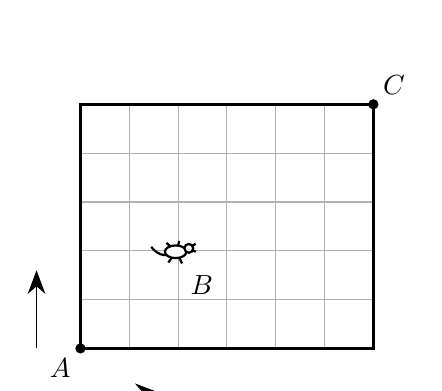
\begin{tikzpicture}[scale=0.62]
            \draw[step=1cm,gray!60] (0,0) grid (6,5);
            \draw[line width=1pt] (0,0) rectangle (6,5);

            \fill (0,0) circle (3pt) node[below left]{$A$};
            \fill (6,5) circle (3pt) node[above right]{$C$};

            \draw[-{Stealth[length=3mm]}] (0,-0.9) -- (1.6,-0.9);
            \draw[-{Stealth[length=3mm]}] (-0.9,0) -- (-0.9,1.6);

            
            \begin{scope}[shift={(2,2)}]
                \draw[thick] (-0.05,-0.05) .. controls (-0.3,-0.15) and (-0.45,-0.05) .. (-0.55,0.08);
                \draw[thick,fill=white] (-0.05,-0.02) ellipse (0.22 and 0.13);
                \draw[thick,fill=white] (0.22,0.05) circle (0.09);
                \draw[thick] (0.28,0.1) -- (0.36,0.14);
                \draw[thick] (0.28,0.02) -- (0.36,-0.02);
                \draw[thick] (-0.12,-0.13) -- (-0.2,-0.24);
                \draw[thick] (0.02,-0.13) -- (0.08,-0.26);
                \draw[thick] (-0.14,0.08) -- (-0.24,0.16);
                \draw[thick] (0.0,0.1) -- (0.02,0.2);
            \end{scope}
            \node[below right=1pt] at (2,1.75) {$B$};
        \end{tikzpicture}
    \end{minipage}
\end{question}

\begin{solution}
    求从 $A(0,0)$ 只能向右或向上沿格线前进，避开 $B(2,2)$ 到达 $C(6,5)$ 的路径总数。\\
    用排除法：先求 $A$ 到 $C$ 的全部路径数，再减去经过 $B$（即被壁虎挡住）的路径数。\\
    $A\to C$ 的全部路径：向右走 $6$ 步，向上走 $5$ 步，共 $11$ 步：
    \[
        \binom{11}{5} = 462
    \]
    经过 $B$ 的路径数（$A\to B$ 再 $B\to C$）：
    \[
        \binom{4}{2}\times\binom{7}{3} = 6\times35 = 210
    \]
    避开 $B$ 的路径数：
    \[
        462-210 = 252
    \]
    故选 A。
\end{solution}
%endregion

%region 范围：高中/大学代数——分数指数的二项式定理（广义二项式展开） | 考点：广义二项式系数 $\binom{n}{r}=\dfrac{n(n-1)(n-2)\cdots(n-r+1)}{r!}$（$n$ 为分数）及展开式中变量项系数的完整计算（含符号与幂次） | 难度：中等偏难
\begin{question}
    求 $\dfrac{1}{\sqrt{1-4x}}$ 展开式中 $x^2$ 的系数。 \paren[D]
    \begin{choices}
        \item $-2$
        \item $2$
        \item $-24$
        \item $24$
    \end{choices}
\end{question}

\begin{solution}
    求 $\dfrac{1}{\sqrt{1-4x}}=(1-4x)^{-\frac12}$ 展开式中 $x^2$ 项的系数。\\
    利用广义二项式定理 $(1+u)^n=\displaystyle\sum_{r=0}^{\infty}\binom{n}{r}u^r$（$\binom{n}{r}=\dfrac{n(n-1)\cdots(n-r+1)}{r!}$），取 $n=-\dfrac12,\ u=-4x,\ r=2$。
    \begin{align*}
        \binom{-\frac12}{2} &= \dfrac{\left(-\frac12\right)\left(-\frac12-1\right)}{2!} \\
        &= \dfrac{\left(-\frac12\right)\left(-\frac32\right)}{2} = \dfrac38
    \end{align*}
    该项为：
    \begin{align*}
        \binom{-\frac12}{2}(-4x)^2 &= \dfrac38\times16x^2 \\
        &= 6x^2
    \end{align*}
    故 $x^2$ 项的系数为 $6$。
\end{solution}
%endregion

%region 范围：高中数学-极限 | 考点：根式极限（分子有理化） | 难度：中等
\begin{question}
    求极限 $\displaystyle\lim_{x\to+\infty}\left(\sqrt{x^2+3x+1}-x\right)$ 的值为 \paren[B]
    \begin{choices}
        \item $3$
        \item $\dfrac{3}{2}$
        \item $\dfrac{1}{2}$
        \item $0$
    \end{choices}
\end{question}

\begin{solution}
    求 $\displaystyle\lim_{x\to+\infty}\left(\sqrt{x^2+3x+1}-x\right)$。\\
    分子有理化，乘以共轭表达式后再除以 $x$ 化简。\\
    \begin{align*}
        \sqrt{x^2+3x+1}-x
        &= \frac{\left(\sqrt{x^2+3x+1}-x\right)\left(\sqrt{x^2+3x+1}+x\right)}{\sqrt{x^2+3x+1}+x} \\
        &= \frac{3x+1}{\sqrt{x^2+3x+1}+x} \\
        &= \frac{3+\dfrac{1}{x}}{\sqrt{1+\dfrac{3}{x}+\dfrac{1}{x^2}}+1}
    \end{align*}
    \[
        \lim_{x\to+\infty}\left(\sqrt{x^2+3x+1}-x\right)
        = \frac{3+0}{\sqrt{1+0+0}+1} = \frac{3}{2}
    \]
    故选 B。
\end{solution}
%endregion

%region 范围：高中/大学微积分——导数定义的极限式变形 | 考点：利用导数定义 $f'(0)=\lim_{h\to0}\dfrac{f(h)-f(0)}{h}$ 对含伸缩变量（如 $2x$）及正负号颠倒的极限式进行换元化简 | 难度：中等
\begin{question}
    已知 $f'(0)=2$，则 $\displaystyle\lim_{x\to0}\dfrac{f(0)-f(2x)}{x}$ 的值为 \paren[C]
    \begin{choices}
        \item $2$
        \item $4$
        \item $-4$
        \item $-2$
    \end{choices}
\end{question}

\begin{solution}
    已知 $f'(0)=2$，求 $\displaystyle\lim_{x\to0}\dfrac{f(0)-f(2x)}{x}$ 的值。\\
    将分子的正负号与自变量 $2x$ 调整为导数定义的标准形式 $\dfrac{f(h)-f(0)}{h}$（其中 $h=2x\to0$），再对照已知的 $f'(0)$ 代入。
    \begin{align*}
        \lim_{x\to0}\dfrac{f(0)-f(2x)}{x} &= \lim_{x\to0}\left[-\dfrac{f(2x)-f(0)}{2x}\times2\right] \\
        &= -2\lim_{x\to0}\dfrac{f(2x)-f(0)}{2x}
    \end{align*}
    令 $h=2x$，当 $x\to0$ 时 $h\to0$：
    \begin{align*}
        -2\lim_{h\to0}\dfrac{f(h)-f(0)}{h} &= -2f'(0) \\
        &= -2(2) = -4
    \end{align*}
    故选 C。
\end{solution}
%endregion

%region 范围：高中/大学微积分——定积分的对称性质 | 考点：利用代换 $x\to a-x$ 结合函数对称条件 $f(x)=f(a-x)$ 求出 $\displaystyle\int_0^a xf(x)\,dx$ 与 $\displaystyle\int_0^a f(x)\,dx$ 的关系 | 难度：中等偏难
\begin{question}
    若 $f(x)=f(a-x)$，则 $\displaystyle\int_0^a xf(x)\,dx$ 的值为 \paren[A]
    \begin{choices}
        \item $\dfrac{a}{2}\displaystyle\int_0^a f(x)\,dx$
        \item $a\displaystyle\int_0^a f(x)\,dx$
        \item $\displaystyle\int_0^a f(x)\,dx$
        \item $\dfrac{1}{2}\displaystyle\int_0^a f(x)\,dx$
    \end{choices}
\end{question}

\begin{solution}
    已知 $f(x)=f(a-x)$，求 $\displaystyle\int_0^a xf(x)\,dx$ 的值。\\
    设 $I=\displaystyle\int_0^a xf(x)\,dx$，对该积分作代换 $x\to a-x$，再利用已知条件将其化回含 $I$ 的方程求解。\\
    设 $I=\displaystyle\int_0^a xf(x)\,dx$，令 $x=a-u$，$dx=-du$：
    \begin{align*}
        I &= \int_0^a (a-u)f(a-u)\,du \\
        &= \int_0^a (a-u)f(u)\,du \qquad (\because f(a-u)=f(u)) \\
        &= a\int_0^a f(u)\,du - \int_0^a uf(u)\,du \\
        &= a\int_0^a f(x)\,dx - I
    \end{align*}
    移项求解：
    \begin{align*}
        2I &= a\int_0^a f(x)\,dx \\
        I &= \dfrac{a}{2}\int_0^a f(x)\,dx
    \end{align*}
    故选 A。
\end{solution}
%endregion

%region 范围：高中/大学复数——棣莫弗定理（De Moivre's Theorem）| 考点：由 $z=\cos\theta+i\sin\theta$ 结合棣莫弗定理求 $z^n+\dfrac{1}{z^n}$ 型表达式（需注意 $\dfrac1z=\cos\theta-i\sin\theta$ 而非直接取倒数保留虚部符号） | 难度：中等
\begin{question}
    设 $z=\cos\theta+i\sin\theta$，则 $z^5+\dfrac{1}{z^5}$ 的值为 \paren[A]
    \begin{choices}
        \item $2\cos5\theta$
        \item $2i\sin5\theta$
        \item $\cos5\theta$
        \item $2\cos\theta$
    \end{choices}
\end{question}

\begin{solution}
    已知 $z=\cos\theta+i\sin\theta$，求 $z^5+\dfrac{1}{z^5}$ 的值。\\
    先用棣莫弗定理求出 $z^5$，再利用 $|z|=1$ 得出 $\dfrac{1}{z}=\cos\theta-i\sin\theta$，从而求出 $\dfrac{1}{z^5}$，两者相加消去虚部。\\
    由棣莫弗定理：
    \[
        z^5 = (\cos\theta+i\sin\theta)^5 = \cos5\theta+i\sin5\theta
    \]
    由 $|z|=1$，$\dfrac1z=\overline{z}=\cos\theta-i\sin\theta$，同理：
    \[
        \dfrac{1}{z^5} = \cos5\theta-i\sin5\theta
    \]
    两式相加：
    \[
        z^5+\dfrac{1}{z^5} = (\cos5\theta+i\sin5\theta)+(\cos5\theta-i\sin5\theta) = 2\cos5\theta
    \]
    故选 A。
\end{solution}
%endregion

%region 范围：解析几何——圆锥曲线（移轴双曲线的准线方程） | 考点：标准式双曲线经平移后的准线公式 $x=h\pm\dfrac{a^2}{c}$，需注意先求 $c=\sqrt{a^2+b^2}$ 再代入中心坐标平移 | 难度：中等
\begin{question}
    双曲线 $\dfrac{(x-2)^2}{16}-\dfrac{(y+1)^2}{9}=1$ 的准线方程为 \paren[A]
    \begin{choices}
        \item $x=\dfrac{26}{5}$ 或 $x=-\dfrac{6}{5}$
        \item $x=\dfrac{16}{5}$ 或 $x=-\dfrac{16}{5}$
        \item $x=\dfrac{19}{5}$ 或 $x=\dfrac{1}{5}$
        \item $x=7$ 或 $x=-3$
    \end{choices}
\end{question}

\begin{solution}
    求双曲线 $\dfrac{(x-2)^2}{16}-\dfrac{(y+1)^2}{9}=1$ 的准线方程。\\
    先由标准式读出 $a^2,b^2$ 及中心坐标，求出 $c$，再代入准线公式 $x=h\pm\dfrac{a^2}{c}$（$h$ 为中心的横坐标）。\\
    设中心为 $(h,k)=(2,-1)$，$a^2=16,\ b^2=9$。
    \begin{align*}
        c &= \sqrt{a^2+b^2} = \sqrt{16+9} = 5
    \end{align*}
    \begin{align*}
        x &= h\pm\dfrac{a^2}{c} \\
        &= 2\pm\dfrac{16}{5}
    \end{align*}
    \[
        x=\dfrac{26}{5} \quad \text{或} \quad x=-\dfrac{6}{5}
    \]
    故选 A。
\end{solution}
%endregion

%region 范围：高中数学-复数与方程 | 考点：立方根的单位根、指数化简 | 难度：中等
\begin{question}
    已知 $x^2+x+1=0$，则 $\displaystyle x^{100}+\frac{1}{x^{10}}$ 的值为 \paren[A]
    \begin{choices}
        \item $-1$
        \item $1$
        \item $2$
        \item $0$
    \end{choices}
\end{question}

\begin{solution}
    已知 $x^2+x+1=0$，求 $\displaystyle x^{100}+\frac{1}{x^{10}}$ 的值。\\
    两边乘以 $(x-1)$ 化为 $x^3=1$，再对指数取模 $3$ 化简。\\
    \begin{align*}
        (x-1)(x^2+x+1) &= x^3-1 = 0 \\
        x^3 &= 1
    \end{align*}
    \[
        100 = 3\times 33 + 1, \quad 10 = 3\times 3 + 1
    \]
    \begin{align*}
        x^{100} &= x^{99}\cdot x = (x^3)^{33}\cdot x = x \\
        \frac{1}{x^{10}} &= x^{-10} = x^{-9}\cdot x^{-1} = (x^3)^{-3}\cdot x^{-1} = x^{-1} = x^2
    \end{align*}
    \[
        x^{100}+\frac{1}{x^{10}} = x + x^2 = -1
    \]
    故选 A。
\end{solution}
%endregion

% %region 范围：复数——根的性质（共轭根定理与根与系数的关系）| 考点：实系数多项式方程的虚根成共轭对出现（共轭根定理），结合根与系数关系（Vieta's Formulas）求未知系数 | 难度：中等偏难
% \begin{question}
%     已知实系数方程 $x^3+ax^2+bx+10=0$ 的其中一个根为 $1-2i$，则 $a$ 的值为 \paren[A]
%     \begin{choices}
%         \item $0$
%         \item $2$
%         \item $-2$
%         \item $4$
%     \end{choices}
% \end{question}

% \begin{solution}
%     已知实系数方程 $x^3+ax^2+bx+10=0$ 的一根为 $1-2i$，求 $a$ 的值。\\
%     由共轭根定理，实系数多项式方程的虚根必成共轭对出现，故 $1+2i$ 也是方程的根；设第三根为实数 $r$，利用根与系数的关系（各根之积、各根之和）求出 $r$ 与 $a$。\\
%     由共轭根定理，另一根为 $1+2i$。设第三根为 $r$（$r\in\mathbb{R}$）。\\
%     由 Vieta 公式，三根之积 $=-\dfrac{10}{1}=-10$：
%     \begin{align*}
%         (1-2i)(1+2i)\cdot r &= -10 \\
%         (1+4)\cdot r &= -10 \\
%         r &= -2
%     \end{align*}
%     由 Vieta 公式，三根之和 $=-a$：
%     \begin{align*}
%         (1-2i)+(1+2i)+(-2) &= -a \\
%         0 &= -a \\
%         a &= 0
%     \end{align*}
%     故选 A。
% \end{solution}
% %endregion

\newpage



%region 范围：高中/大学函数——反三角函数图像的伸缩变换 | 考点：识别 $y=2\arccos x$ 图像的定义域、值域（$[0,2\pi]$）及单调性，并与"漏乘系数""方向反射""定义域平移"等常见错误图像区分 | 难度：中等偏难
\begin{question}
    下列哪一个是 $y=2\cos^{-1}x$ 的函数图像？（非等比例真实尺度） \paren[A]
    \begin{choices}
        \item
        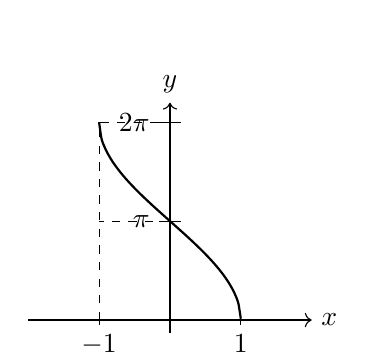
\begin{tikzpicture}[xscale=0.9,yscale=0.4]
            \draw[->] (-2,0) -- (2,0) node[right]{$x$};
            \draw[->] (0,-0.4) -- (0,6.9) node[above]{$y$};
            \draw[dashed] (-1,0) -- (-1,6.2832) -- (0,6.2832);
            \draw[dashed] (0,3.14159) -- (-1,3.14159);
            \draw (-1,0.15) -- (-1,-0.15) node[below]{$-1$};
            \draw (1,0.15) -- (1,-0.15) node[below]{$1$};
            \draw (0.15,6.2832) -- (-0.15,6.2832) node[left]{$2\pi$};
            \draw (0.15,3.14159) -- (-0.15,3.14159) node[left]{$\pi$};
            \draw[thick,domain=-1:1,smooth,samples=60,variable=\x]
                plot ({\x},{2*acos(\x)*3.14159/180});
        \end{tikzpicture}

        \item
        \begin{tikzpicture}[xscale=0.9,yscale=0.4]
            \draw[->] (-2,0) -- (2,0) node[right]{$x$};
            \draw[->] (0,-0.4) -- (0,6.9) node[above]{$y$};
            \draw[dashed] (-1,0) -- (-1,3.14159) -- (0,3.14159);
            \draw (-1,0.15) -- (-1,-0.15) node[below]{$-1$};
            \draw (1,0.15) -- (1,-0.15) node[below]{$1$};
            \draw (0.15,3.14159) -- (-0.15,3.14159) node[left]{$\pi$};
            \draw[thick,domain=-1:1,smooth,samples=60,variable=\x]
                plot ({\x},{acos(\x)*3.14159/180});
        \end{tikzpicture}

        \item
        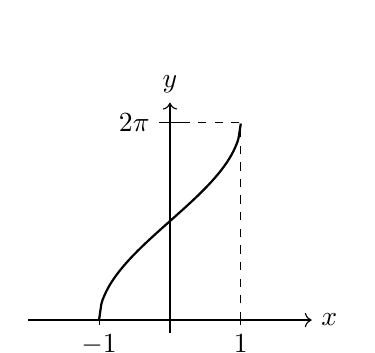
\begin{tikzpicture}[xscale=0.9,yscale=0.4]
            \draw[->] (-2,0) -- (2,0) node[right]{$x$};
            \draw[->] (0,-0.4) -- (0,6.9) node[above]{$y$};
            \draw[dashed] (1,0) -- (1,6.2832) -- (0,6.2832);
            \draw (-1,0.15) -- (-1,-0.15) node[below]{$-1$};
            \draw (1,0.15) -- (1,-0.15) node[below]{$1$};
            \draw (0.15,6.2832) -- (-0.15,6.2832) node[left]{$2\pi$};
            \draw[thick,domain=-1:1,smooth,samples=60,variable=\x]
                plot ({\x},{2*acos(-\x)*3.14159/180});
        \end{tikzpicture}

        \item
        \begin{tikzpicture}[xscale=0.9,yscale=0.4]
            \draw[->] (-1,0) -- (3,0) node[right]{$x$};
            \draw[->] (0,-0.4) -- (0,6.9) node[above]{$y$};
            \draw[dashed] (0,0) -- (0,6.2832);
            \draw[dashed] (1,3.14159) -- (0,3.14159);
            \draw (0.05,0.15) -- (0.05,-0.15) node[below]{$0$};
            \draw (2,0.15) -- (2,-0.15) node[below]{$2$};
            \draw (0.15,6.2832) -- (-0.15,6.2832) node[left]{$2\pi$};
            \draw (0.15,3.14159) -- (-0.15,3.14159) node[left]{$\pi$};
            \draw[thick,domain=0:2,smooth,samples=60,variable=\x]
                plot ({\x},{2*acos(\x-1)*3.14159/180});
        \end{tikzpicture}
    \end{choices}
\end{question}

\begin{solution}
    判断 $y=2\cos^{-1}x$（即 $y=2\arccos x$）的正确图像。\\
    先确定定义域、值域与单调性：$\arccos x$ 定义域为 $[-1,1]$，值域为 $[0,\pi]$，乘以系数 $2$ 后值域伸缩为 $[0,2\pi]$，且 $\arccos$ 本身为减函数，图像应为递减。\\
    代入关键点验证：
    \begin{align*}
        x=-1:\ y&=2\arccos(-1)=2\pi \\
        x=0:\ y&=2\arccos(0)=\pi \\
        x=1:\ y&=2\arccos(1)=0
    \end{align*}
    图像应在 $x\in[-1,1]$ 上由 $(-1,2\pi)$ 递减经过 $(0,\pi)$ 到达 $(1,0)$，与选项 A 相符（选项 B 漏乘系数 $2$，值域仍为 $[0,\pi]$；选项 C 方向反射成递增；选项 D 定义域错误平移为 $[0,2]$）。
    故选 A。
\end{solution}
%endregion

%region 范围：高中数学-多项式与因式分解 | 考点：换元法因式分解、单位根性质 | 难度：中等
\begin{question}
    下列何者不是 $x^{36} - 4x^9 + 3$ 的因式？\paren[C]
    \begin{choices}
        \item $x-1$
        \item $x^2+x+1$
        \item $x^3+1$
        \item $x^6+x^3+1$
    \end{choices}
\end{question}

\begin{solution}
    判断各选项是否整除 $x^{36}-4x^9+3$。\\
    令 $t=x^9$，将原式化为关于 $t$ 的多项式后因式分解。\\
    设 $t=x^9$，
    \begin{align*}
        t^4 - 4t + 3 &= (t-1)^2(t^2+2t+3) \\
        x^{36}-4x^9+3 &= (x^9-1)^2\left(x^{18}+2x^9+3\right)
    \end{align*}
    再将 $x^9-1$ 因式分解：
    \begin{align*}
        x^9 - 1 &= (x^3-1)(x^6+x^3+1) \\
        &= (x-1)(x^2+x+1)(x^6+x^3+1)
    \end{align*}
    故 $x-1$、$x^2+x+1$、$x^6+x^3+1$ 均为因式；而 $x^3+1=(x+1)(x^2-x+1)$ 中 $x=-1$ 不满足 $(-1)^9=1$，故 $x+1$（进而 $x^3+1$）不是 $x^9-1$ 的因式，也不是原式的因式。
    故选 C。
\end{solution}
%endregion


% %region 范围：空间向量——向量内积（数量积）及夹角 | 考点：向量内积的坐标计算公式与夹角公式 $\cos\theta=\dfrac{\vec{a}\cdot\vec{b}}{|\vec{a}||\vec{b}|}$，需正确区分内积为零（垂直）与内积符号所反映的夹角性质 | 难度：中等
% \begin{question}
%     已知向量 $\vec{a}=(2,-1,2)$，$\vec{b}=(1,2,-2)$，则 $\vec{a}$ 与 $\vec{b}$ 的夹角为 \paren[C]
%     \begin{choices}
%         \item $\dfrac{\pi}{6}$
%         \item $\dfrac{\pi}{3}$
%         \item $\dfrac{2\pi}{3}$
%         \item $\dfrac{5\pi}{6}$
%     \end{choices}
% \end{question}

% \begin{solution}
%     求向量 $\vec{a}=(2,-1,2)$ 与 $\vec{b}=(1,2,-2)$ 的夹角。\\
%     先用坐标公式求出内积 $\vec{a}\cdot\vec{b}$ 及各自的模，再代入夹角公式求出 $\theta$。
%     \begin{align*}
%         \vec{a}\cdot\vec{b} &= 2(1)+(-1)(2)+2(-2) \\
%         &= 2-2-4 = -4
%     \end{align*}
%     \begin{align*}
%         |\vec{a}| &= \sqrt{2^2+(-1)^2+2^2}=\sqrt{9}=3 \\
%         |\vec{b}| &= \sqrt{1^2+2^2+(-2)^2}=\sqrt{9}=3
%     \end{align*}
%     \begin{align*}
%         \cos\theta &= \dfrac{\vec{a}\cdot\vec{b}}{|\vec{a}||\vec{b}|} = \dfrac{-4}{3\times3} = -\dfrac{4}{9}
%     \end{align*}
%     由 $\cos\theta=-\dfrac49<0$，可知 $\theta$ 为钝角，对照选项中 $\cos\dfrac{2\pi}{3}=-\dfrac12$ 与 $\cos\dfrac{5\pi}{6}=-\dfrac{\sqrt3}{2}$，$-\dfrac49$ 更接近 $-\dfrac12$：
%     \[
%         \theta \approx \dfrac{2\pi}{3}
%     \]
%     故选 C。
% \end{solution}

% %endregion


\vfill % 与上方内容保持距离

\noindent
\newlength{\sigwidth}
\settowidth{\sigwidth}{（\hspace{4em}师）}

\begin{tabular*}{\textwidth}{@{\extracolsep{\fill}} l l l}
    出题： & 审题： & 审核： \\[4em]
    \rule{\sigwidth}{0.5pt} &
    \rule{\sigwidth}{0.5pt} &
    \rule{\sigwidth}{0.5pt} \\
    （\hspace{0em} \setterteacher ） &
    （\hspace{0em} \reviewteacher ）  &
    （\hspace{0em} \auditteacher ） \\
\end{tabular*}

\clearpage
\thispagestyle{empty} % 取消这一页的页眉页脚（页码）
~
\clearpage
\end{document}
